\documentclass[10pt, twocolumn, twoside]{article}

\usepackage{graphicx}
\usepackage{amsmath, amssymb}
\usepackage{enumerate}
\usepackage{titleps}
\usepackage[top=0.75in,bottom=0.75in,right=0.5in,left=0.5in]{geometry}
\usepackage[parfill]{parskip}
\usepackage{titling}
\usepackage{hyperref}
\newcommand{\squeezeup}{\vspace{-2.5mm}}
\usepackage{lipsum, babel}
\hypersetup{
    colorlinks=true,
    linkcolor=blue,
    filecolor=magenta,      
    urlcolor=cyan,
}

\graphicspath{ {../images/}, {timimages/} }


\newpagestyle{ruled}
{\setfoot{}{\thepage}{} \footrule}
\pagestyle{ruled}


\setlength{\droptitle}{-4em}   % This is your set screw

\title{6.867 Project: Comparing Methods for Low-Data Image Segmentation}
\date{December 12, 2017}
\author {Kimberly Villalobos Carballo, Timothy Leplae-Arthur, Sean Fraser}


\begin{document}
\maketitle

\begin{abstract}
\squeezeup
In this paper we explore various image segmentation techniques. Specifically, we compare and analyze two different methods for image segmentation \cite{Kaur}: Edge Detection and Clustering. For these implementations we are using the Berkeley Segmentation Dataset and Benchmarks 500 (\href{https://www2.eecs.berkeley.edu/Research/Projects/CS/vision/grouping/resources.html}{BSDS500}) which consists of 500 natural images. For each image, several people were asked to draw a contour map separating different objects based on their own understanding. Using these human-drawn segmentations as the ground truth, we evaluated four different approaches to segmentation by edge detection and clustering: edge-based segmentation from a Convolutional Neural Network (CNN), color-based clustering segmentation on both a pixel-level and super-pixel-level, and finally a new method involving using both the edge map from the CNN and a super-pixel assignment. To compare the performance of these approaches, we measured Precision / Recall on detected segment boundaries in addition to three other region-based metrics.  We conclude that the edge-based segmentation from the CNN performs the best.

\end{abstract}

\section{Introduction}
\squeezeup
\squeezeup
Segmentation partitions an image into constituent non-overlapping regions or objects, that correlate strongly with objects or features of interest in the image. Precisely, image segmentation is the process of assigning a label to every pixel in the image such that pixels with the same label share certain characteristics. Segmentation is an important problem with several applications in fields such as medical imaging, object detection, and recognition tasks.

Image segmentation has been widely recognized as a difficult task \cite{Arbelaez, Kaur} and unsupervised segmentation often results in unsatisfactory results. Recent approaches to segmentation involve both classical clustering based approaches which often perform best on images where segments are well-defined by color dissimilarity \cite{Arbelaez}, as well as contour and edge-based methods that first frame edge-detection as a supervised learning problem with neural networks\cite{El-Sayed}. With this in mind, we sought to compare and explore the performance of different approaches, and look at the strengths and weaknesses of each. Common direct segmentation techniques involve non-parametric methods such as clustering techniques, however depending on the image at hand, can have very poor results, especially if two separate and far apart sections of the image had very similar colors for example. By introducing the supervised edge-detection method using neural networks, to first get an edge boundary and then attempt to get a segmentation from the edge map, we looked to see how using boundaries can improve or exacerbate segmentations. To this end, we explored in depth how convolutional neural network architectures can affect edge-detection and therefore segmentation results, in addition to the traditional clustering methods using both normal pixels and superpixel methods \cite{Bergh}. 

Finally, noticing that both clustering and edge-based detection methods had their respective advantages and disadvantages, we tried a new approach involving combining the edge map from the neural network with the super pixel segmentation, in an attempt to more accurately segment the images. We found that this novel approach lead to improvements on some images, but worse results on others.

\section{Dataset}
\squeezeup
\squeezeup
To compare our implementations and explore our hypotheses, we used the Berkeley Segmentation Dataset and Benchmarks 500 (\href{https://www2.eecs.berkeley.edu/Research/Projects/CS/vision/grouping/resources.html}{BSDS500}) which consists of 500 natural images. Each natural image is on average segmented by five different human subjects. In addition to the raw images and ground truth labels consisting of the collection of human-marked boundaries, the dataset also provided benchmarks and performance metrics. In general, the performance is measured upon how well the boundaries are defined and how well the segmented regions are defined. 

\section{Overview}
\squeezeup
\squeezeup
There are several steps to achieving our four different segmentation results, which include several different parts and pre and post-processing steps. The work flow is summarized in Figure \ref{fig:workflow}. 

\begin{figure}[ht]
	\centering
	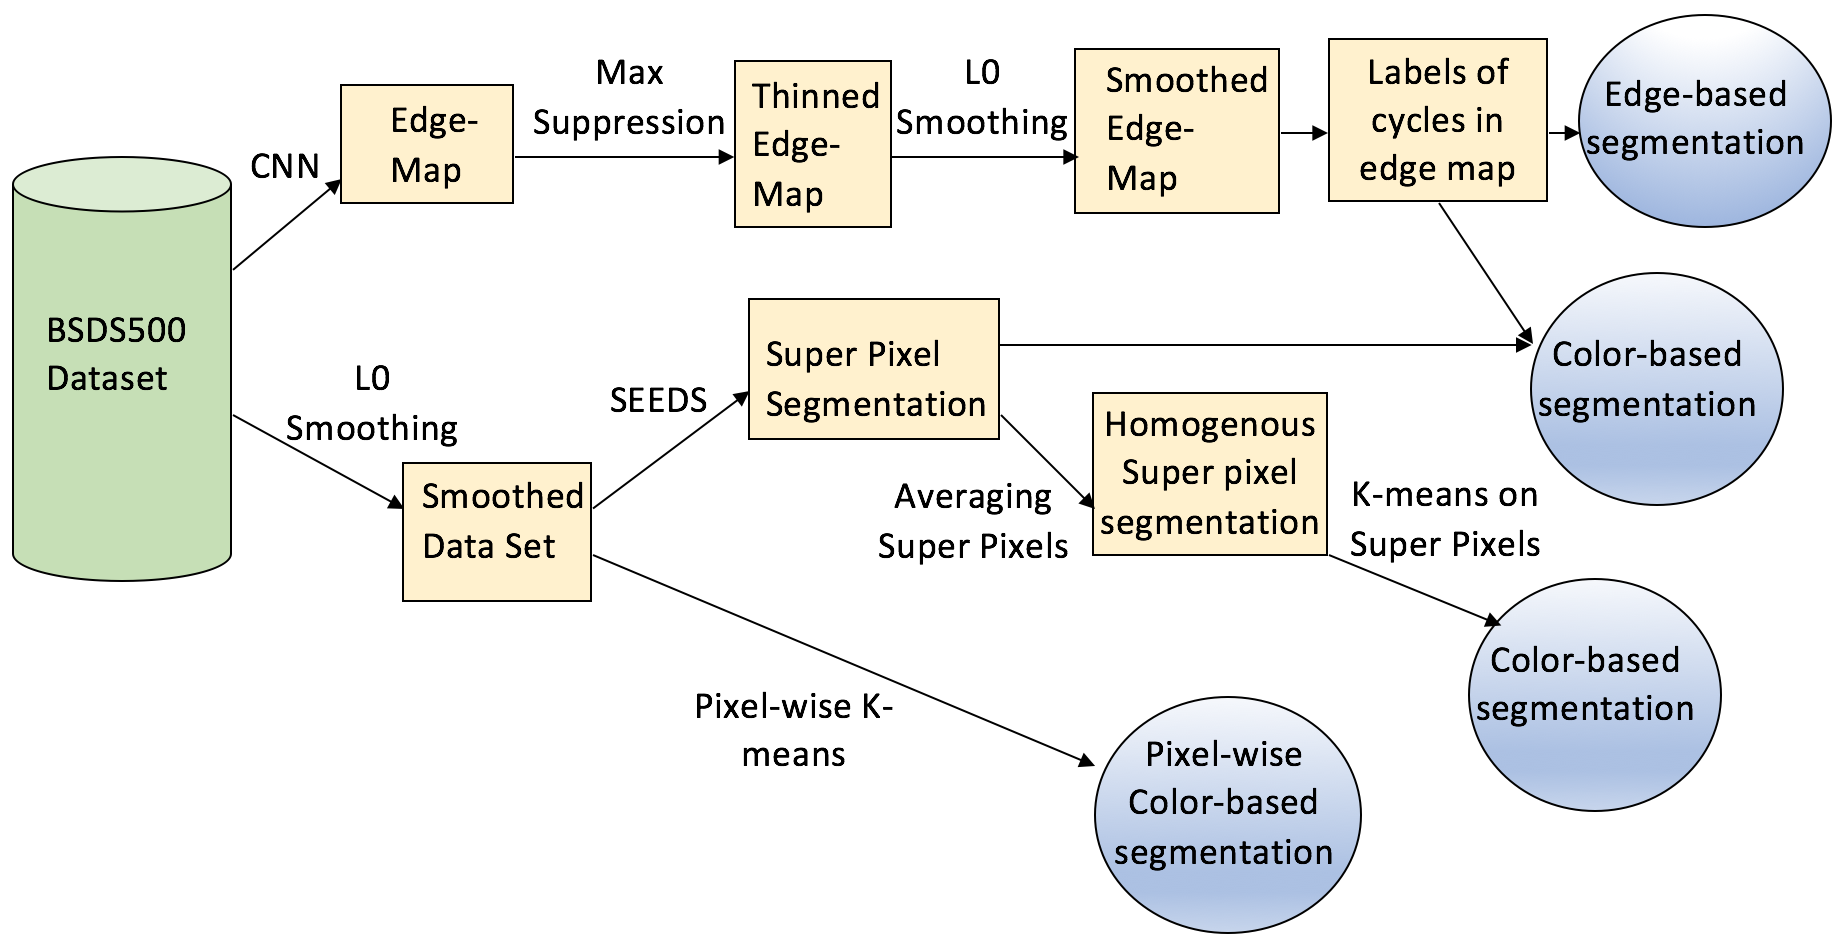
\includegraphics[width=3.6in]{workflow}
    \caption{Work flow that produces our four different segmentation results.}
    \label{fig:workflow}
\end{figure}


Our first model implements edge-based segmentation. We use a neural network to find the edge map of each image, then we apply different post processing techniques to improve the boundaries and finally the edges are divided into loops that are later filled and numbered to obtain the segmented image.

Since segmentation through neural networks is not a common technique, we also developed a segmentation model that relies on a more common approach: color similarity. We pre-processed the data, and then applied an existing implementation of K-Means to cluster pixels and super-pixels based on how similar their colors are.

Lastly, we looked at a model that combines both pieces of information: the edge map and the color-based clustering. By first encapsulating the color dependencies through super-pixels we can later fill the loops of the edge map with clusters of pixels instead of single pixels. 

We compare all four results at the end using a few different metrics. For measuring how good the segmentation boundaries are we use the F-measure, defined as 
\[F=2\times\frac{\text{precision}\times \text{recall}}{\text{precision}+\text{recall}}\]where \textit{precision} is the probability that a machine-generated boundary pixel is a true boundary pixel and \textit{recall} is the probability that a true boundary pixel is detected (\href{https://www2.eecs.berkeley.edu/Research/Projects/CS/vision/grouping/resources.html}{BSDS500}).

Additionally, we use three different metrics to test the quality of the regions in the segmentation. The first one is Ground-Truth Covering metric based on PASCAL evaluation code \cite{Everingham}. Second is the Variation of Information Index, which measures the distance between two segmentations. Lastly we also measured our results with the Probabilistic Rand Index, which quantifies similarities between clusterings.

\section{CNN}
\squeezeup
\squeezeup
In general, there are a few different methods to segment subjects using a neural network approach. Here, we look at fast, accurate, and data-efficient algorithms that can compare with non-parametric methods. While Semantic Segmentation is a popular method for accurate segmentation, we decided not to pursue it, due to its inefficient use of data, and slow inference. Instead, we choose a method based on the assumption that detecting the edge of the subject can assist in subsequent non-parametric segmentation. Since edges are formed in many different ways, there is no single detection rule that we can objectivize in our model, making this task difficult. Conventional models assume that color and intensity change drastically at the edge between different objects, and remain the same within the interior of the same object. Of course, this is not true. Hence this is why we decide to pursue an approach that learns to detect edges based on man-made labeled data. 

\subsection{Model}
\squeezeup

In Figure \ref{fig:2}, we provide a general layout of our model, which we train with varying parameters. The input of our convolutional neural network is a single image. Before every pooling layer is a branching layer that reconstructs an edge map of our image. The output of our model is a linear combination of these branched edge maps (whose parameters are also learned in the model).

%There should be a figure here that describes the overview of the network
\begin{figure}[h]
    \centering 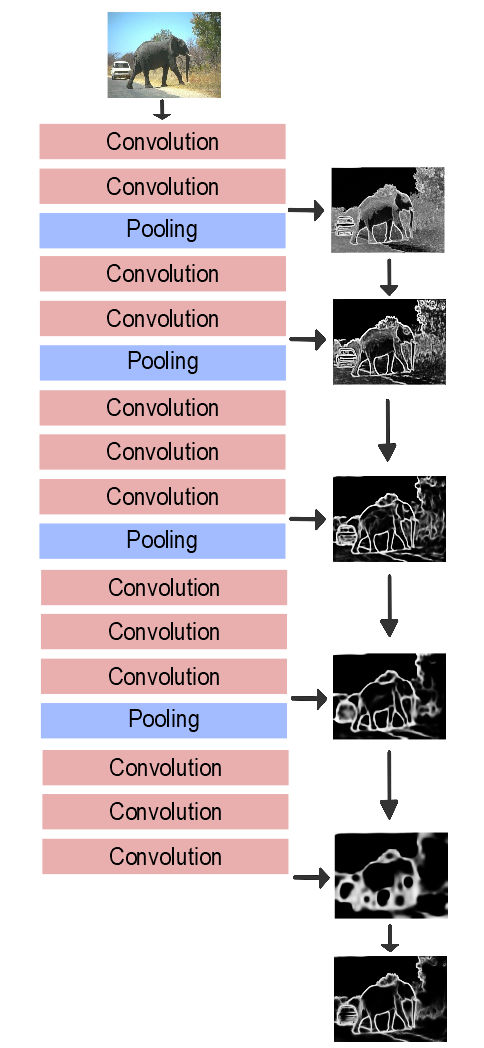
\includegraphics[height=4.0in]{model_overview}
    \caption{Overview of the model}
    \label{fig:2}
\end{figure}
\squeezeup
\squeezeup

\subsection{Training and Data}
\squeezeup
The BSD500 data set is pre-partitioned into a training, validation, and test set with sizes 200, 100, and 200, respectively. We trained all of our models using the \texttt{cuda-convet} toolbox on a GTX 1060 GPU for 100 epochs, which sufficiently achieves minimal training error. The training process lasts about 1.5 hours for all models. To make our model more robust to scaling, translations, or reflections to input data, for each image, we augment our training data to include four random combinations of these transformations with random parameters. 

\subsection{Architecture}
\squeezeup
The general model of the convolutional neural network described in Figure \ref{fig:2} is the main skeleton of our system.  Even with this skeleton, choosing the best parameters is not straightforward, especially when training is expensive. To select the best model, we follow a greedy approach on a few main parameters; namely, the kernel size and the pooling function. 

\subsection{CNN Results}
\squeezeup
We first tested our model with varying kernel sizes: 2, 3, 4. The best performance was achieved with a 3x3 kernel. Figures $\ref{fig:kern_train_error}$, $\ref{fig:kern_val_acc}$, $\ref{fig:kern_entrop}$ show the training error, validation accuracy, and cross-entropy with respect to these three kernel sizes, which are represented by the colors blue, orange, and red respectively. As shown by comparison, the 3x3 kernel achieves best performance, followed by the 2x2 kernel. 

%comparing different kernel sizes

\begin{figure}[h]
    \centering
    \begin{subfigure}
        \centering
        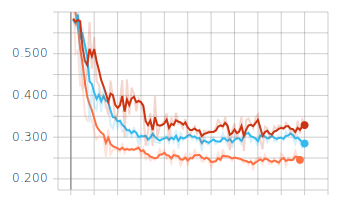
\includegraphics[height=1.2in]{kern_train_error}
        \caption{Training error for varying kernel sizes}
        \label{fig:kern_train_error}
    \end{subfigure}
    \vspace{3mm}
    \begin{subfigure}
        \centering
        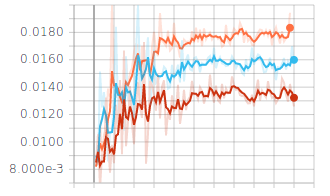
\includegraphics[height=1.2in]{kern_val_acc}
        \caption{Val. acc. for varying kernel sizes}
        \label{fig:kern_val_acc}
    \end{subfigure}
    \vspace{3mm}
    \begin{subfigure}
        \centering
        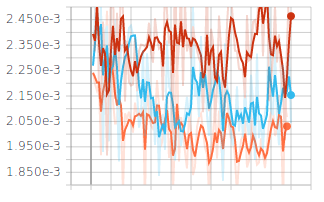
\includegraphics[height=1.2in]{kern_entrop}
        \caption{Cross-entropy for varying kernel sizes}
        \label{fig:kern_entrop}
    \end{subfigure}
    \label{fig:different_kernel}
\end{figure}


% \begin{figure}[h]
%     \centering
%     \begin{subfigure}
%         \centering
%         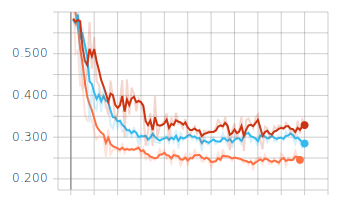
\includegraphics[height=1.2in]{kern_train_error}
%         \caption{Training error per epoch}
%         \label{fig:kern_train_error}
%     \end{subfigure}
%     \hfill
%     \begin{subfigure}
%         \centering
%         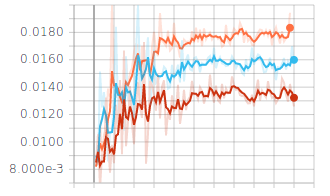
\includegraphics[height=1.2in]{kern_val_acc}
%         \caption{Val. acc. per epoch}
%         \label{fig:kern_val_acc}
%     \end{subfigure}
%     \hfill
%     \begin{subfigure}
%         \centering
%         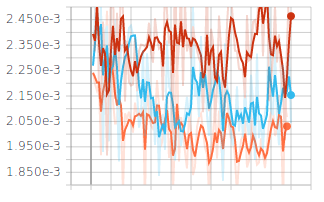
\includegraphics[height=1.2in]{kern_entrop}
%         \caption{Cross-entropy per epoch}
%         \label{fig:kern_entrop}
%     \end{subfigure}
%     \caption{2x2 kernel: blue, 3x3 kernel: orange, 4x4 kernel: red}
%     \label{fig:different_kernel}
% \end{figure}

We also test our model using a Max Pooling layer and an Average Pooling Layer. Figures $\ref{fig:pool_train}$, $\ref{fig:pool_val}$, $\ref{fig:pool_x}$ show the performance of the Max Pooling and Average Pooling functions, represented by orange and blue respectively. Here, the cross-entropy is only slightly lower for the Max Pooling layer, but this marginal difference is supported by the substantially improved performance in validation accuracy and training error. 

%comparing different pooling
\begin{figure}[h]
    \centering
    \begin{subfigure}
        \centering
        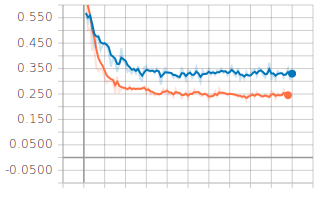
\includegraphics[height=1.2in]{pool_train_error}
        \caption{Training error for varying pooling functions}
        \label{fig:pool_train}
    \end{subfigure}
    \vspace{3mm}
    \begin{subfigure}
        \centering
        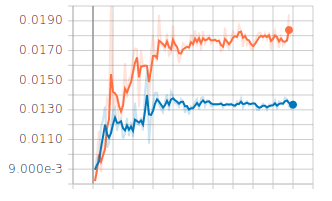
\includegraphics[height=1.2in]{pool_val_acc}
        \caption{Val. acc. for varying pooling functions}
        \label{fig:pool_val}
    \end{subfigure}
    \vspace{3mm}
    \begin{subfigure}
        \centering
        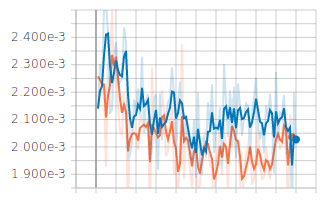
\includegraphics[height=1.2in]{pool_entrop}
        \caption{Cross-entropy for varying pooling functions}
        \label{fig:pool_x}
    \end{subfigure}
    \label{fig:10}
\end{figure}

As we would expect, these different choices of parameters can lead to significantly different inferred edge maps. Figure \ref{fig:15} shows the different edge maps, on an example image from our test set. We can see that among all the parameter combinations tested, the Max Pooling architecture with 3x3 kernel produces an edge map with highest contrast between interiors and edges which is consistent with its highest performance on validation accuracy. In general, without any nontrivial optimization, inference on a 420x320 image takes ~1.3 secs (stdev: .1), which is significantly less than semantic segmentation. 

% In the Figure below, we illustrate the varying edge maps for the respective choice of parameters. 

\begin{figure}[h!]
    \centering
    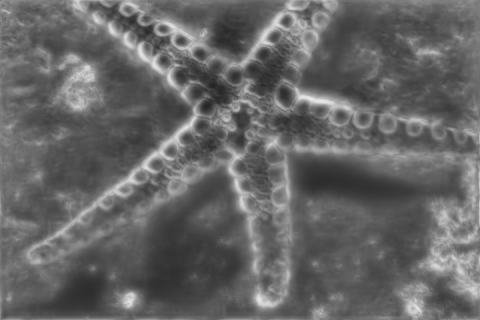
\includegraphics[height=1.2in]{12003_out_orig}
    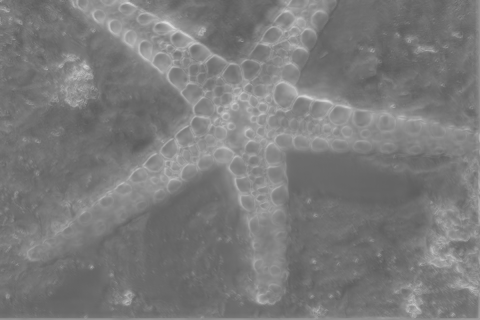
\includegraphics[height=1.2in]{12003_out_2kern}
    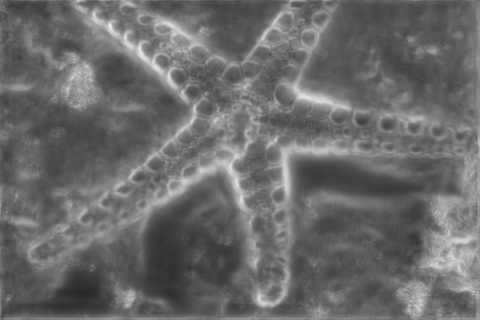
\includegraphics[height=1.2in]{12003_out_4kern}
    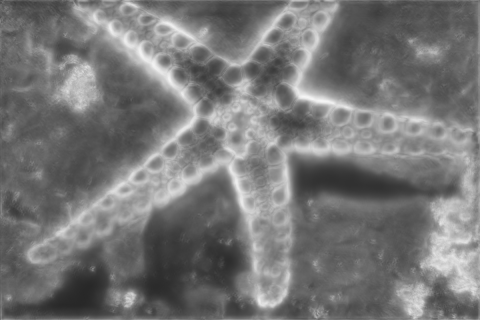
\includegraphics[height=1.2in]{12003_out_avg}
    \caption{Inferred edge maps with varying parameters: 3x3 kernel with MaxPooling, 2x2 kernel with MaxPooling, 4x4 kernel with MaxPooling, 3x3 kernel with AveragePooling}
    \label{fig:15}
\end{figure}


% \begin{figure}[h!]
%     \centering
%     \begin{subfigure}
%         \centering
%         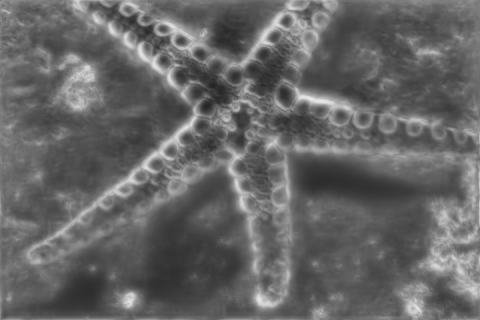
\includegraphics[height=1.2in]{12003_out_orig}
%         \caption{3x3 kernel with Max Pooling Layers}
%     \end{subfigure}
%     \begin{subfigure}
%         \centering
%         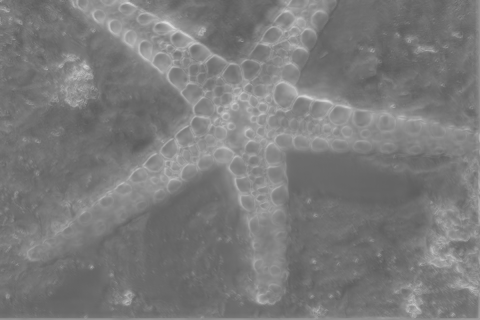
\includegraphics[height=1.2in]{12003_out_2kern}
%         \caption{2x2 kernel with Max Pooling Layers}
%     \end{subfigure}
%     \begin{subfigure}
%         \centering
%         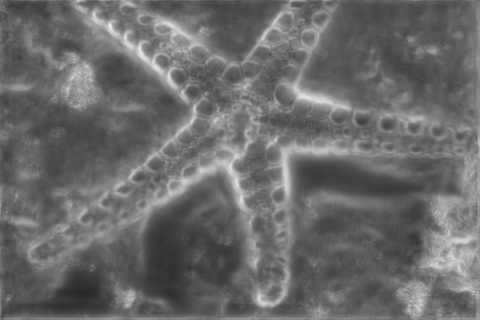
\includegraphics[height=1.2in]{12003_out_4kern}
%         \caption{4x4 kernel with Max Pooling Layers}
%     \end{subfigure}
%     \begin{subfigure}
%         \centering
%         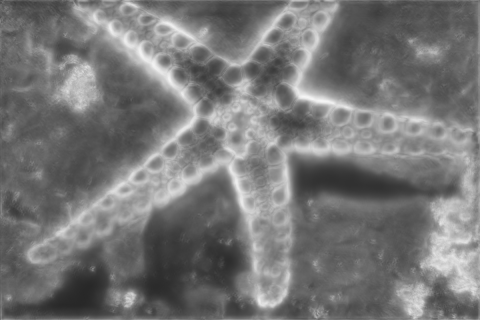
\includegraphics[height=1.2in]{12003_out_avg}
%         \caption{3x3 kernel with Average Pooling Layers}
%     \end{subfigure}
%     \label{fig:15}
% \end{figure}
\squeezeup
\squeezeup
\subsection{Post Processing the Data}
\squeezeup
With these choice of parameters, we apply a post-processing step to prepare the edge map for a better setting for segmentation inference. Often, the edges detected by the convolutional neural network cover several pixels, which is inaccurate. In this regard, we apply a morphological operation to thin the edges of the final output in the data. Figure $\ref{fig:11}$ illustrates the effect of this operation on an example output.

\begin{figure}[h!]
    \centering
    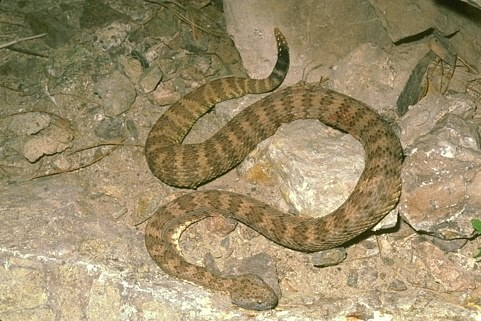
\includegraphics[height=1.2in]{morph_orig}
    \vspace{5mm}
    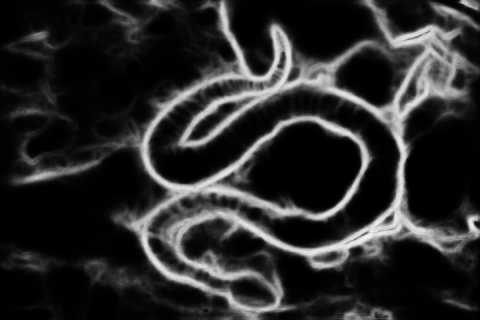
\includegraphics[height=1.2in]{morph_cnn_out}
    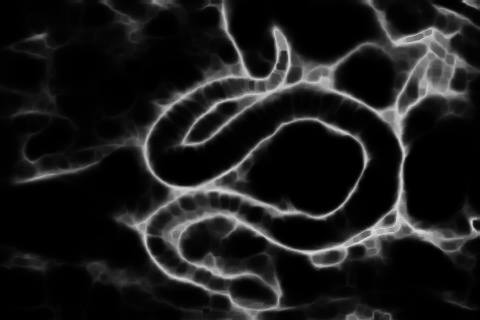
\includegraphics[height=1.2in]{morph_morph}
    \caption{Above, we show the original image, the edge map outputted by the CNN, and the output of applying the morphological operation.}
    \label{fig:11}
\end{figure}


% \begin{figure}[h!]
%     \centering
%     \begin{subfigure}
%         \centering
%         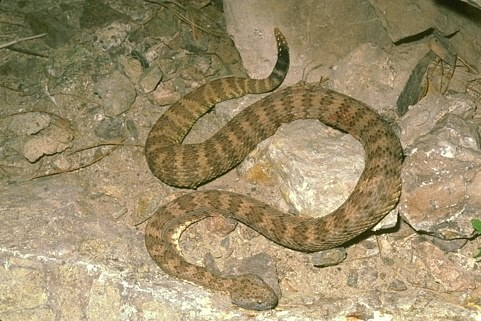
\includegraphics[height=1.2in]{morph_orig}
%         \caption{Original Image}
%     \end{subfigure}
%     \begin{subfigure}
%         \centering
%         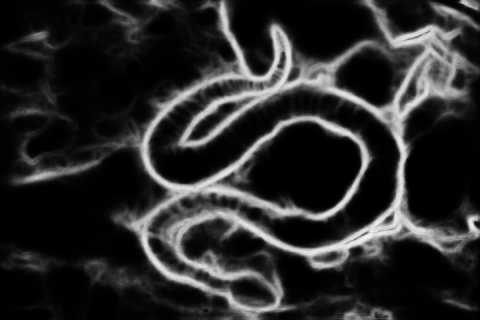
\includegraphics[height=1.2in]{morph_cnn_out}
%         \caption{CNN output}
%     \end{subfigure}
%     \begin{subfigure}
%         \centering
%         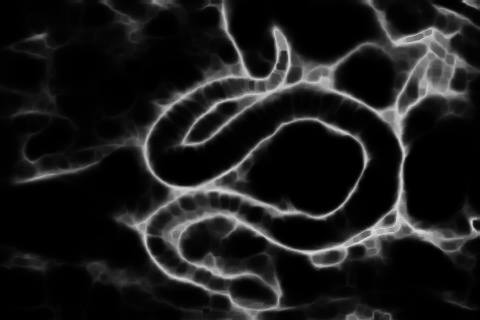
\includegraphics[height=1.2in]{morph_morph}
%         \caption{Final output (after morphing)}
%     \end{subfigure}
%     \caption{Morphing the output of the CNN creates finer edges}
%     \label{fig:5}
% \end{figure}

The precise morphological operation we used is erosion, which is a simple operation that strips away a layer of pixels less than a fixed margin from a boundary region. Here, a 3x3 kernel yielded the best results.

% Tim's part

% Post processing max suppression
% Post processing with L0 
% Image thinning and loop finding for segmentation (video)

\subsection{From edge-map to segmentation}
\squeezeup
\begin{figure}[ht]
    \centering
    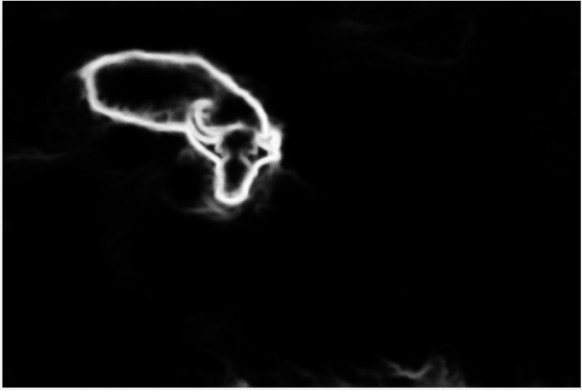
\includegraphics[width=1.5in]{thin1}
    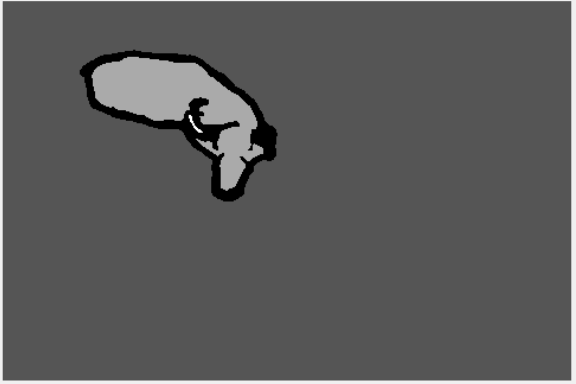
\includegraphics[width=1.5in]{thin2}
    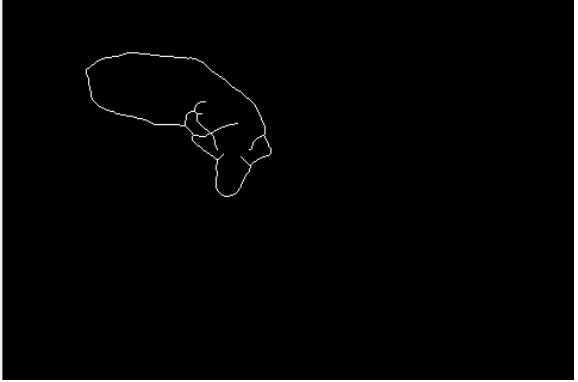
\includegraphics[width=1.5in]{thin3}
    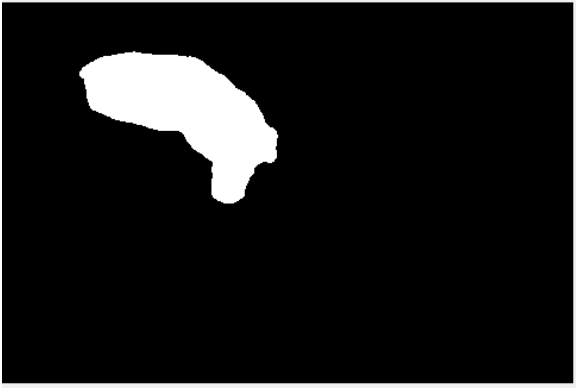
\includegraphics[width=1.5in]{thin4}    
    \caption{Comparison of the output edge map of the CNN (top left), the segmentation based on that output with no post-processing (top right), the result of edge thinning on the edge map (bottom left), and finally the segmentation based on the thinner edge map after post-processing (bottom right), for a sample image.}
    \label{fig:thinning}
\end{figure}

To get the segmented image using only the edge-map output from the neural network, we first reduced the boundaries to minimal width and next find the cycles that determine each individual segment. For that we first nullified those pixels whose value in the gray scale was below a certain threshold, and then we applied MATLAB morphological operations to thin the edges obtained from the output of the neural network. This technique removes pixels so that an object without holes shrinks to a minimally connected stroke, and an object with holes shrinks to a connected ring halfway between each hole and the outer boundary. We then fill each cycle and output them all as different segments. As we can observe in Figure \ref{fig:thinning}, if we had not fully reduced the edge width, the border itself would have been classified as a cycle, resulting in the boundaries being classified as another segment.

Figure \ref{fig:reg32} shows the trade-off caused by the threshold we choose. When the threshold is very small, the noise from the edge map creates many small cycles all over the image, causing over segmentation. On the contrary, when the threshold is too big, many pixels are set to zero, which could destroy some of the cycles and damage the segmentation results.

\begin{figure}[h!]
    \centering
    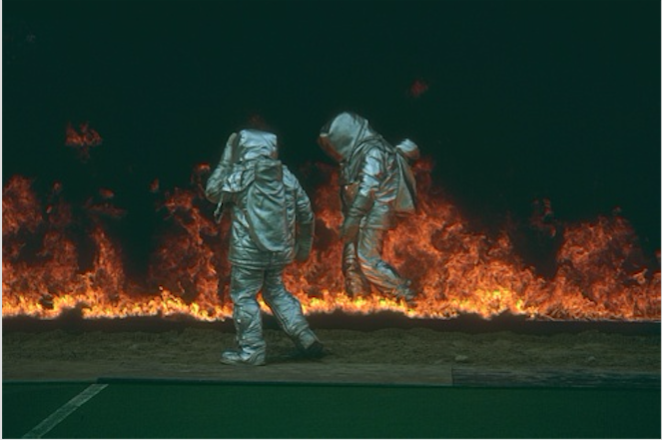
\includegraphics[width=1.5in]{285022}
    \newline
    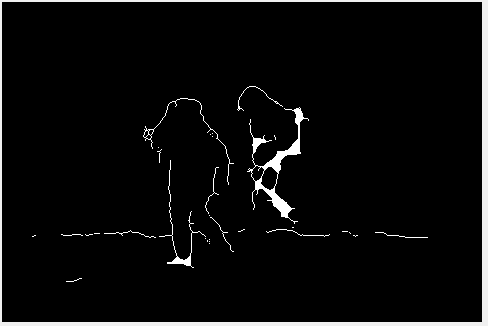
\includegraphics[width=1.5in]{images/285022_large_t.png}
    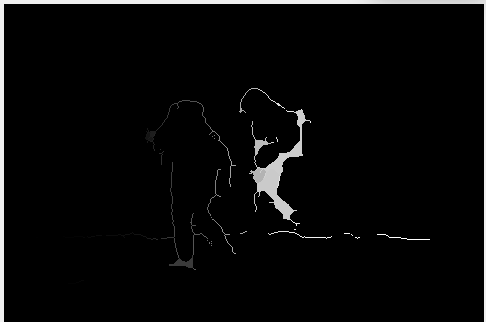
\includegraphics[width=1.5in]{images/285022_small_t.png}
    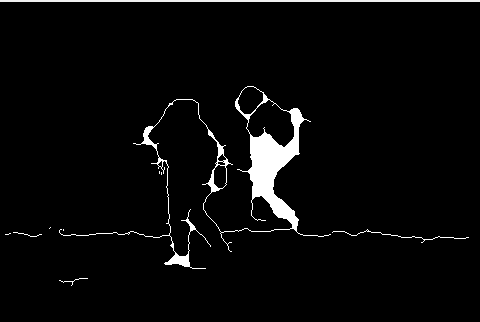
\includegraphics[width=1.5in]{images/285022_high_t.png}
    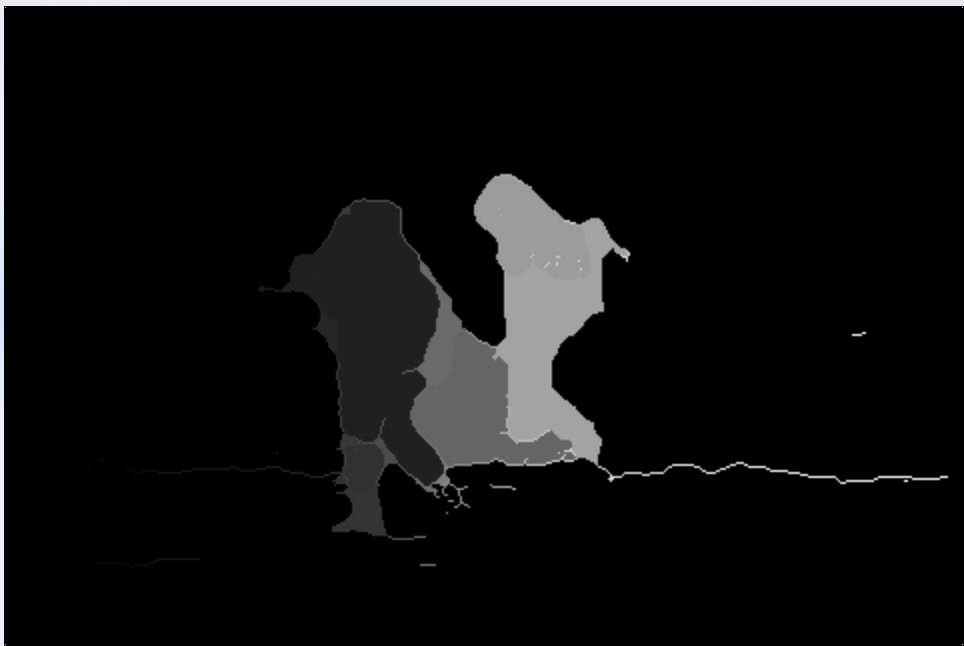
\includegraphics[width=1.5in]{images/285022_little_l.png}
    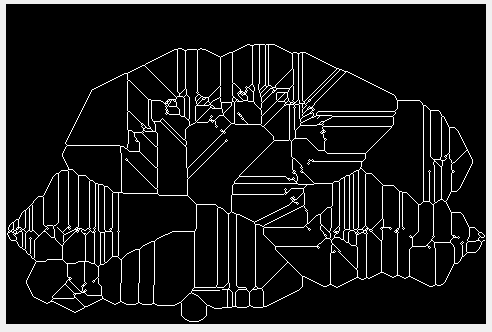
\includegraphics[width=1.5in]{images/285022_low_t.png}
    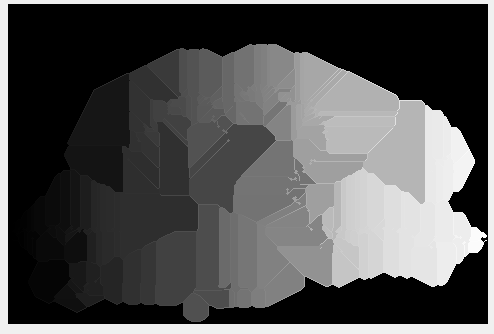
\includegraphics[width=1.5in]{images/285022_many_l.png}

    \caption{Results of segmentation with different thresholds for thinning. The first column shows the edge map after applying the threshold and second column has the corresponding loops found. The first, second and third rows show results for thresholds of 0.4, 0.2 and 0.1 respectively, where the input image had gray-scale in [0,1]. Watch the process \href{https://www.dropbox.com/s/2548p86sl9sgzq8/Segmentation.mov?dl=0}{here}. }
    \label{fig:reg32}
\end{figure}

\subsection{Segmentation Results}
\squeezeup
Table \ref{table:segresults1} below shows that this model has significantly higher Precision than Recall. When the edge map returned by the neural network has a lot of noise, it becomes hard for the segmentation algorithm to find loops in the boundaries; however, most loops identified accurately represent boundaries for a segment of the image. These results support each other, since high precision indicates that the segments found by the model accurately represented segments of the ground truth data, while lower recall tells us that a significant part of the segments were missing in the output. Additionally, all other metrics indicate that the similarity between the regions of the ground truth and the output segmentations were not as significant as that of the boundaries.

% \begin{center}
%  \begin{tabular}{||c c c c c c||} 
%  \hline
%  GT Covering & R.I & V.I & Recall & Precision & F\\ [0.5ex] 
%  \hline\hline
%  0.42 & 0.57 & 2.32 & 0.59 & 0.72 & 0.65\\ 
%  \hline
% \end{tabular}
% \end{center}

\begin{table}[ht]
\caption{Comparison of results, using several measures} % title of Table
\centering % used for centering table
\begin{tabular}{c c c c c c} % centered columns (4 columns)
\hline\hline %inserts double horizontal lines
GT Covering & R.I. & V.O.I. & Recall & Precision & F \\ [0.5ex] % inserts table
%heading
\hline % inserts single horizontal line % [1ex] adds vertical space
 0.42 & 0.57 & 2.32 & 0.59 & 0.72 & 0.65 \\ 
\hline %inserts single line
\end{tabular}
\label{table:segresults1} % is used to refer this table in the text
\end{table}

\begin{figure}[h]
	\centering
	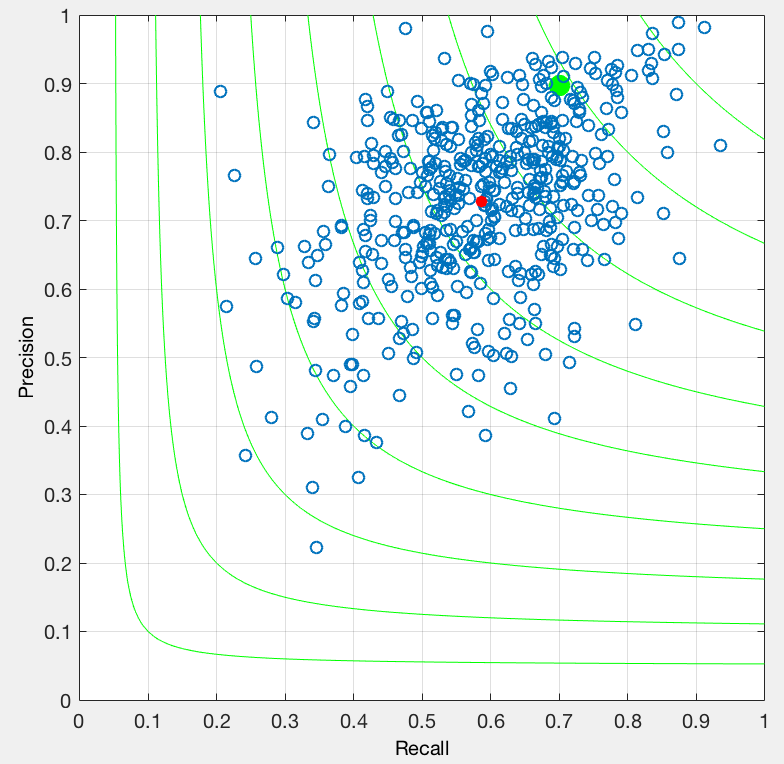
\includegraphics[width=2.3in]{images/F-NN.png}
    \caption{Precision-Recall for edge-based model. The green dot represents performance by humans, blue dots correspond to the 500 data point and the red point is their total average.}
    \label{fig:F-NN}
\end{figure}

\squeezeup
\section{Color-based Clustering}
\subsection{K-Means at a pixel-level}
\squeezeup
For this method we used MATLAB Statistic and Image Processing toolboxes to implement K-Means clustering on the input images. First the images are converted from RGB to $L*a*b$ color space. Then for a specific $k$ the centers are computed and for each pixel we assign the nearest center using Euclidean distance. This method focuses on minimizing the distance between pixels in the same cluster, and maximizing the distance between pixels in different clusters. The initial centers are chosen randomly and the optimal value for the number of clusters, $k$, is the one that minimizes the sum of square distances between the points and their centers.

\begin{figure}[h!]
    \centering
    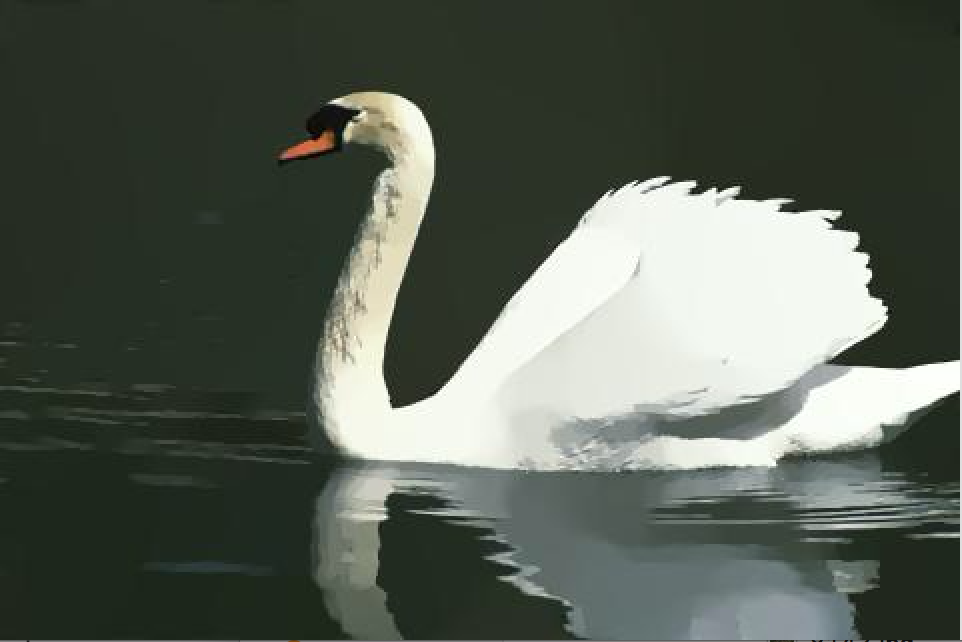
\includegraphics[width=1.5in]{images/8068.png}
    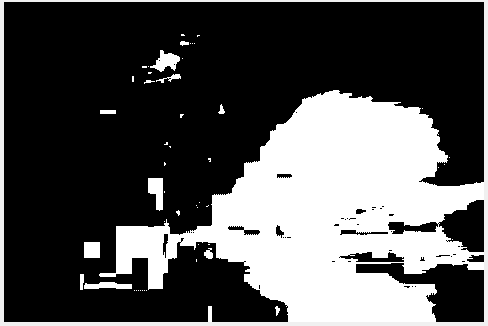
\includegraphics[width=1.5in]{images/k_2.png}
    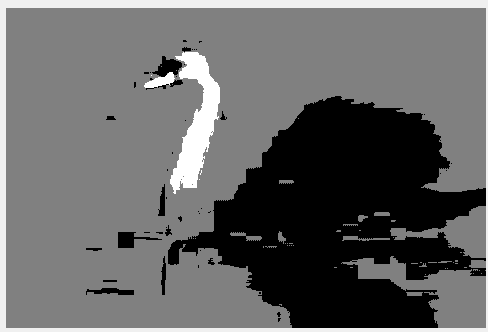
\includegraphics[width=1.5in]{images/k3.png}
    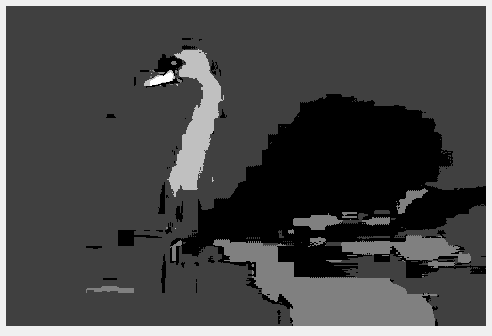
\includegraphics[width=1.5in]{images/k_5.png}

    \caption{Top left is the original image, top right is the segmentation with 2 clusters, bottom left is the segmentation with 3 clusters and bottom right is the segmentation with 5 clusters.}
    \label{fig:reg3}
    \squeezeup
\end{figure}

\subsubsection{Preprocessing}

Natural images, such as the ones in the BSDS500, are often degraded by noise. To this end, we applied a noise reduction algorithm described in \cite{Xu}, that is, Image Smoothing via $L_0$ Gradient Minimization. This algorithm aims to reduce the complexity/ noise of the natural images.
As shown in Figure \ref{fig:reg3}, this method improved the accuracies of the segmentation from our K-Means model by removing noise and making the images more homogeneous before clustering. This method improved the accuracies of the segmentations for our K-means clustering based method but made little or no difference with the CNN based method when used a pre-processing. This is what we expect, as the clustering approach is fairly primitive, so adding this extra layer of processing helps, whereas in the CNN, this may already be handled in some way through the convolutional or pooling layers of the network architecture. The image smoothing works by globally controlling the number of non-zero gradients that result to approximate prominent structure, and controlling and smoothing that. 

\begin{figure}[ht]
    \centering
    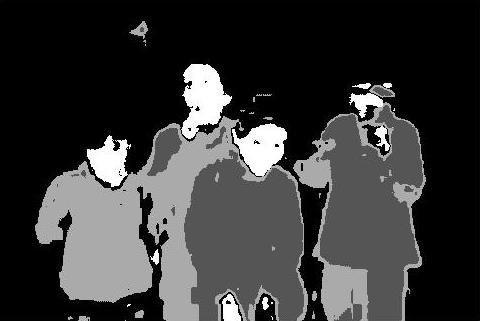
\includegraphics[width=1.5in]{290035_k4_l0}
    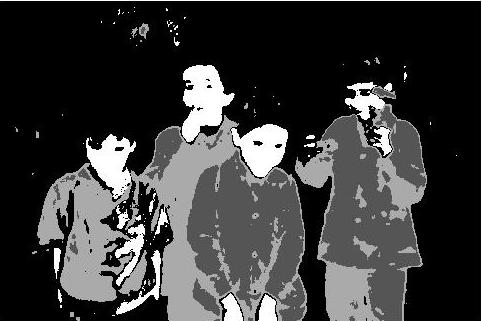
\includegraphics[width=1.5in]{290035_k4}
    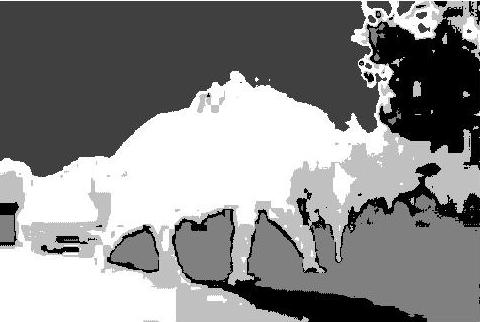
\includegraphics[width=1.5in]{296028_k5_l0}
    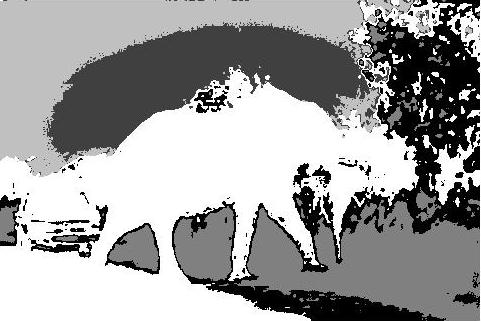
\includegraphics[width=1.5in]{296028_k5}
    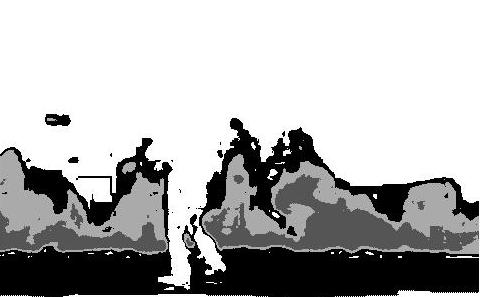
\includegraphics[width=1.5in]{285022_k4_l0}
    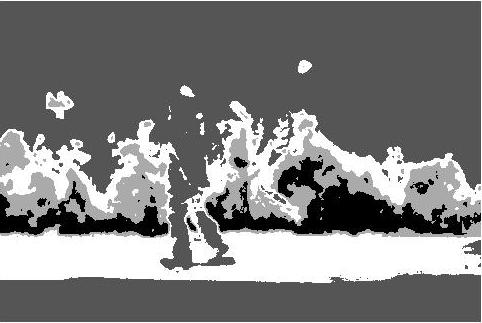
\includegraphics[width=1.5in]{285022_k4}

    \caption{Results of Image Smoothing on our clustering on three different images. The left column shows results of the clustering algorithm after image smoothing / denoising. The right column is the result of the clustering on the original image.}
    \label{fig:reg3}
\end{figure}

Even though this model does very well on images whose objects all have very different colors, it gives poor results when different objects have the exact same or similar pixel values (see Figure \ref{fig:reg33}). Contrary to the results obtained with edge-based segmentations, this model has a high average \texit{recall} but a low average \textit{precision} (see Table \ref{table:table_k}). This suggests that the model performed well finding most of the segments, but also found significantly more segments than those in the ground truth segmentations. Additionally, the values for the GT covering and the other metrics are very close to those obtained in the previous section, indicating that the neural network approach outperforms this clustering method mostly on the boundaries detected.

\begin{figure}[h!]
    \centering
    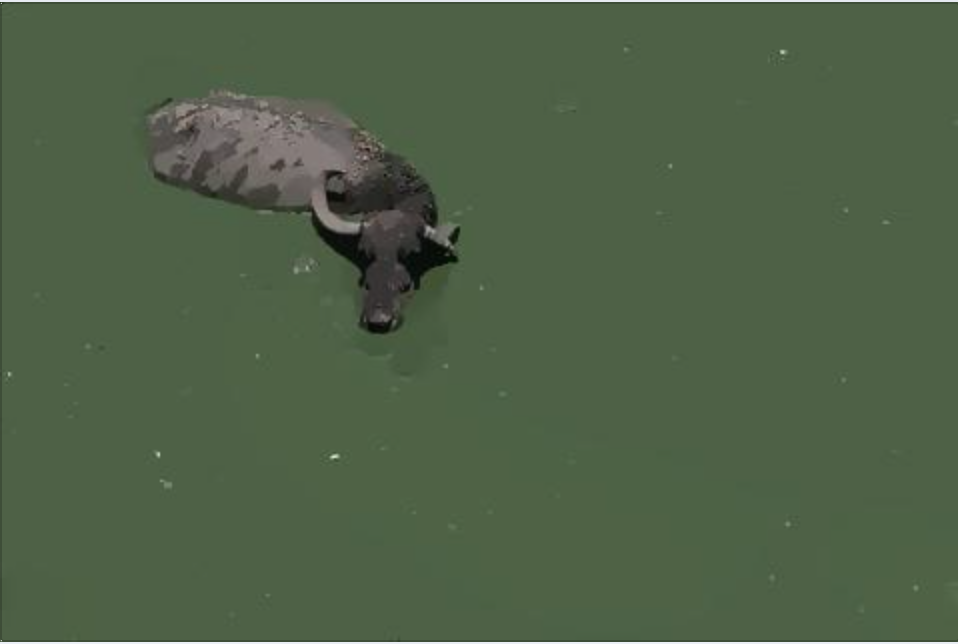
\includegraphics[width=1.5in]{images/80099.png}
    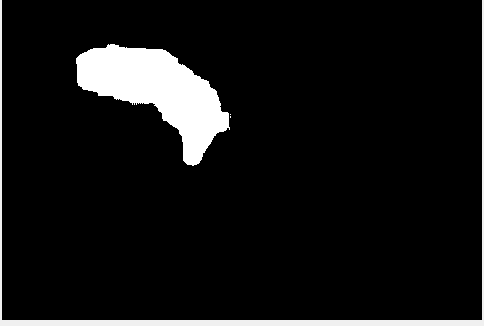
\includegraphics[width=1.5in]{images/80099k.png}
    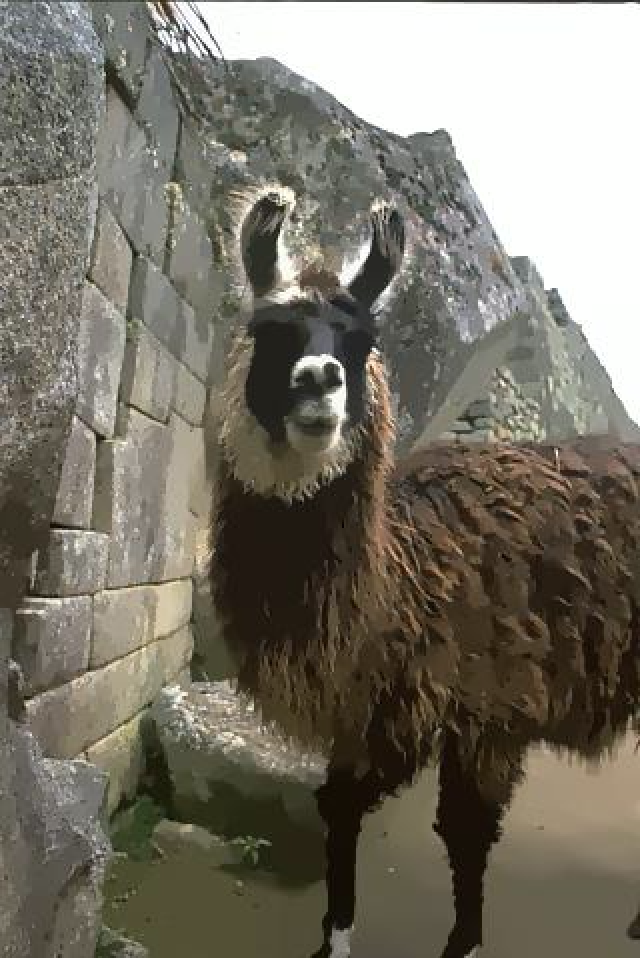
\includegraphics[width=1.5in]{images/6046.png}
    \includegraphics[width=1.5in]{images/6046k.png}

    \caption{First column shows the original image and second column the results from K-Means segmentation.}
    \label{fig:reg33}
\end{figure}

% \begin{center}
% \caption{Comparison of results, using several measures (R.I. is RandIndex, V.O.I. is Variation of Information measures)}
% \label{fig:table_k}
%  \begin{tabular}{||c c c c c c||} 
%  \hline
%  GT Covering & R.I & V.I & Recall & Precision & F \\ [0.5ex] 
%  \hline\hline
%  0.41 & 0.66 & 2.54 & 0.61& 0.38 & 0.47\\ 
%  \hline
% \end{tabular}
% \end{center}

\begin{table}[ht]
\caption{Results} % title of Table
\centering % used for centering table
\begin{tabular}{c c c c c c} % centered columns (4 columns)
\hline\hline %inserts double horizontal lines
GT Covering & R.I. & V.O.I. & Recall & Precision & F \\ [0.5ex] % inserts table
%heading
\hline % inserts single horizontal line % [1ex] adds vertical space
 0.41 & 0.66 & 2.54 & 0.61 & 0.38 & 0.47 \\ 
\hline %inserts single line
\end{tabular}
\label{table:table_k} % is used to refer this table in the text
\end{table}

\begin{figure}[h]
	\centering
	\includegraphics[width=2.3in]{images/F-kmeans.png}
    \caption{Precision-Recall for K-Means model. The green dot represents performance by humans, blue dots correspond to the 500 data point and the red point is their total average.}
    \label{fig:F-kmeans}
\end{figure}

\subsection{Clustering Super pixels}
\squeezeup
Super-pixels are an over-segmentation of the image that clusters pixels that belong to the same object. We used the OpenCV SEEDS \cite{Bergh} implementation which starts from an initial partitioning of the super pixels in a grid shape and then continuously modifies the boundaries of the super pixels
by enforcing color similarity between the boundaries and the super pixel color histogram (see Figure \ref{fig:superpixels}).

\begin{figure}[ht]
	\centering
	\includegraphics[width=3.4in]{super_pixels}
    \caption{Sample image showing super-pixels obtained from the SEEDS algorithm.}
    \label{fig:superpixels}
\end{figure}

We again pre-processed the images using $L_0$ minimization \cite{Xu}, and then found the super-pixels. We then replaced the value of each pixel by the average value of the super-pixel containing it in RGB. We can see in Figure \ref{fig:avgsuperpixels} how this procedure makes the colors of the image more homogeneous. Next we applied MATLAB's \texttt{adaptive k-means} \cite{Bhatia} to the averaged super pixels, which clusters color and gray scale images using K-Means without having to specify the value of $k$. 

\begin{figure}[ht]
	\centering
	\includegraphics[width=3.4in]{average_super_pixels}
    \caption{Sample image showing each pixel represented by the average of the super-pixel it belongs to from our implementation.}
    \label{fig:avgsuperpixels}
\end{figure}

From looking at Table \ref{table:table_j} below we notice that the indices for evaluating the regions of our segmentation are quite similar to those obtained in the previous implementation of \texttt{k-means} on the pixels of the image, however there is an important difference on the boundary metrics. The \textit{recall} is lower and the \textit{precision} is higher, showing a the trade-off arising between both quantities when clustering is made on super pixels instead of individual pixels. Because both quantities changed a similar amount but in different directions, the \textit{F} score remains almost identical as before.


% \begin{center}
% \label{fig:table_k}
%  \begin{tabular}{||c c c c c c||} 
%  \hline
%  GT Covering & R.I & V.I & Recall & Precision & F\\ [0.5ex] 
%  \hline\hline
%  0.39 & 0.64 & 2.64 & 0.48& 0.47&0.47 \\ 
%  \hline
% \end{tabular}
% \end{center}

\begin{table}[ht]
\caption{Results} % title of Table
\centering % used for centering table
\begin{tabular}{c c c c c c} % centered columns (4 columns)
\hline\hline %inserts double horizontal lines
GT Covering & R.I. & V.O.I. & Recall & Precision & F \\ [0.5ex] % inserts table
%heading
\hline % inserts single horizontal line % [1ex] adds vertical space
 0.39 & 0.64 & 2.64 & 0.48 & 0.47 & 0.47 \\ 
\hline %inserts single line
\end{tabular}
\label{table:table_j} % is used to refer this table in the text
\end{table}

\begin{figure}[ht]
	\centering
	\includegraphics[width=2.3in]{images/F-supixel.png}
    \caption{Precision-Recall for clustering of super-pixels model. The green dot represents performance by humans, blue dots correspond to the 500 data point and the red point is their total average.}
    \label{fig:F-supixel}
\end{figure}

\squeezeup
\section{Combining edges and clusters}
\squeezeup
In this section we explore a final model that mixes both of the methods discussed above. We divide the input image into small clusters based on color similarity; next we place and group such clusters in the edge map like in a Jigsaw puzzle, in such a way that the boundaries of the edge map match as closely as possible the boundaries of the groups formed. 

\begin{figure}[h]
    \centering
    \includegraphics[width=1.5in]{images/eleph.png}
    \includegraphics[width=1.5in]{images/43051.png}
    \includegraphics[width=1.5in]{images/eleph_NN.png}
    \includegraphics[width=1.5in]{images/43051_NN.png}
    
    \includegraphics[width=1.5in]{images/eleph_mix.png}
    \includegraphics[width=1.5in]{images/43051_mix.png}

    \caption{Example of segmentation improved and exacerbated by the combined model. From top to bottom: original image, edge-based only segmentation, combined segmentation.}
    \label{fig:reg37}
\end{figure}

After obtaining the super-pixels for each image, we took the edge map given by the NN implementation and one more time found the loops after thresh-holding and thinning the edges. We then proceeded to fill the loops to find the different segments, but unlike the method used in the neural network approach, this time the loops were filled with super-pixels instead of with pixels, i.e, each super pixel was assigned to be in the same cluster as the cycle that contained the majority of the pixels in the super pixel. The results for one of the images is shown in Figure \ref{fig:reg37}, where we can see that the super pixels helped improve the shape of the elephant.

Unfortunately, this method does not always improve the segmentation results obtained by the first edge-based approach. Whenever the boundaries of the original image are well represented by the super pixels, i.e., when they are perfectly contained in the boundaries of the super pixels, this model improves upon the NN approach alone, since the super pixels improve the boundaries obtained by the edge map. On the other hand, when some of the super pixels incorrectly contain pixels that must belong to different segments, those pixels will continue to be together when placed on the edge map, which could potentially worsen the segmentation obtained when filling the cycles with individual pixels instead (see Figure \ref{fig:reg38}).


\subsection{Results}
 
Table \ref{table:table_l} shows the results obtained for this model. Even though the \textit{precision} is just as high as that obtained by the implementation of neural network edge map without super pixels, the \textit{recall} significantly decreased, which led to a lower $F$ score. This suggests that some of the super pixels did not completely capture the edges of the image, and then when placing the super pixel on the edge map the boundaries from the NN worsened. Lastly, notice that the metrics for region evaluation did not change much, but their slight decrease supports our argument above. Since the super pixels are relatively small, even if its boundaries do not match very well the edge map boundaries, the regions obtained by filling loops with super pixels will not be very different from the regions obtained by filling the loops with single pixels.

% \begin{center}
%  \begin{tabular}{||c c c c c c||} 
%  \hline
%  GT Covering & R.I & V.I & Recall & Precision & F\\ [0.5ex] 
%  \hline\hline
%  0.39 & 0.64 & 2.64 & 0.36& 0.72&0.48 \\ 
%  \hline
% \end{tabular}
% \end{center}

\begin{figure}[h]
\squeezeup
\squeezeup
\squeezeup
	\centering
	\includegraphics[width=2.1in]{images/F-mix.png}
    \caption{Precision-Recall for combined model. The green dot represents performance by humans, blue dots correspond to the 500 data point and the red point is their total average.}
    \label{fig:Fmix}
\end{figure}

\begin{table}[ht]
\caption{Results} % title of Table
\centering % used for centering table
\begin{tabular}{c c c c c c} % centered columns (4 columns)
\hline\hline %inserts double horizontal lines
GT Covering & R.I. & V.O.I. & Recall & Precision & F \\ [0.5ex] % inserts table
%heading
\hline % inserts single horizontal line % [1ex] adds vertical space
 0.39 & 0.64 & 2.64 & 0.36 & 0.72 & 0.48 \\ 
\hline %inserts single line
\end{tabular}
\label{table:table_l} % is used to refer this table in the text
\end{table}

\begin{figure}[h]
\squeezeup
\squeezeup
    \centering
    \includegraphics[width=1.3in]{images/original.png}
    \includegraphics[width=1.3in]{images/gr.png}
    \includegraphics[width=1.3in]{images/NN.png}
    \includegraphics[width=1.3in]{images/kmean.png}
    \includegraphics[width=1.3in]{images/supixel.png}
    \includegraphics[width=1.3in]{images/mix.png}

    \caption{From left to right, top to bottom: original, ground truth, edge-based segmentation only, pixel-level K-Means, super-pixel level K-Means, and the combined model consisting of the edge-map and super-pixel assignment.}
    \label{fig:reg38}
\end{figure}

\section{Conclusions}

After comparing and analyzing the results obtained for all four segmentation outputs we can conclude that the edge-based approach by the neural network without clustering outperforms all other methods. This suggests that the edge map resulting from the CNN produces boundaries that are more accurate than those found through color-based models. Even though none of the methods explored reached very high accuracies, they could all be further improved by tackling problems specific to each model.

In particular, we found that the noise in the edge maps was the main difficulty in our model, since the loops were harder to find when the boundaries were not clearly defined. For future work, it would be interesting to explore other techniques to go from the edge map to the image segmentation that do not rely as much on continuous loops, in addition to trying different pre and post-processing techniques that could improve the quality of the edges output by the neural network.


\section{Division of Labor}

Code is available at: \\
\href{https://github.com/seanfraser/6867-project}{\texttt{https://github.com/seanfraser/6867-project}}.

We roughly divided the work as follows: 
Timothy worked on the neural network implementations as well as maximal suppression for post-processing. Sean worked on the segmentation implementations relying on color-based clustering, as well $L_0$ denoising for pre and post-processing. Kimberly implemented the algorithm to go from the edge map to the image segmentation, the combined model using super pixels and the edge map, and the evaluation of the models. The write up was split equally.

\newpage
\begin{thebibliography}{9}
\bibitem{Arbelaez}
Arbelaez, P.; Maire, M.; Fowlkes, C.; Malik, J. (2011)
``Contour Detection and Hierarchical Image Segmentation"
\textit{IEEE TPAMI} 33.5: 898-916
\bibitem{El-Sayed}
El-Sayed, M.; Estaitia, Y.; Khafagy M. (2013)
``Automated Edge Detection Using Convolutional
Neural Network"
\textit{International Journal of Advanced Computer Science and Applications} 4.10
\bibitem{Xu}
Xu, L.; Lu, C.; Xu, Y.; Jia, J. (2011)
``Image Smoothing via $L_0$
 Gradient Minimization"
\textit{ACM Trans. Graph.} 30.6
\bibitem{Kaur}
Kaur, D.; Kaur, Y. (2014)
``Various Image Segmentation
Techniques: A Review"
\textit{International Journal of Computer Science and Mobile Computing} 3.5: 809-814
\bibitem{Wang}
Wang, R. (2016)
``Edge Detection Using Convolution Neural Network"
\textit{Advances in Neural Networks - ISNN} 20: 741
\bibitem{Bergh}
Van den Bergh, M.; Boix, X.; Roig, G.; Van Gool, L.  (2013)
``SEEDS: Superpixels Extracted via Energy-Driven Sampling"
\textit{ArXiv e-prints} 1309.3848
\bibitem{Xie}
Xie, S.; Tu, Z. (2015)
``Holistically-Nested Edge Detection"
\textit{Proceedings of IEEE International Conference on Computer Vision}
\bibitem{Bhatia}
Bhatia, S. (2004)
``Adaptive K-Means Clustering"
\textit{Flairs Conference, 695-699}
\bibitem{Everingham}
Everingham, M.; Van Gool, L.; Williams, C.; Winn, J.; Zisserman, A. (2010)
``The PASCAL Visual Object Classes (VOC) Challenge"
\textit{Int J Comput Vis} 88: 303-338

\end{thebibliography}

\end{document}